\documentclass[11pt,a4paper]{article}
\usepackage[margin=2.2cm]{geometry}
\usepackage[T1]{fontenc}
\usepackage{lmodern}
\usepackage{microtype}
\usepackage{booktabs}
\usepackage{tabularx}
\usepackage{graphicx}
\usepackage{enumitem}
\usepackage{caption}
\usepackage[hidelinks]{hyperref}
\setlist{itemsep=2pt,topsep=4pt}
\captionsetup{font=small,labelfont=bf}
\newcommand{\code}[1]{\texttt{#1}}

\title{\textbf{Emoji Vendor Classification}\\[2pt]
\large Summary of the methods tried and what we learned}
\author{Erdem Sanver\\\small Computer Vision 2026 -- BSc AIDAMS -- Final Project (team \emph{The Winners})}
\date{18 October 2026}

\begin{document}
\maketitle

\begin{abstract}
\noindent This note summarises every experiment I ran for the Kaggle challenge, including the ones we
did not submit and the ones that failed. In short: starting from the team's 0.788 public score, a
pipeline with correct transparency handling, ImageNet-pretrained ConvNeXt-Tiny fully fine-tuned at
high resolution, retraining on 100\% of the data and a 3-model ensemble reached \textbf{0.981} on
the public leaderboard (4th of 16 teams at our last check). 22 experiments are logged with method,
preprocessing, rationale and scores in \code{results/Strategies Computer Vision Project.xlsx}.
\end{abstract}

\section{Task and evaluation protocol}
Seven classes (apple, google, whatsapp, facebook, samsung, mozilla, messenger), 9\,879 labelled
training PNGs and 9\,879 test PNGs; metric = accuracy. The classes are imbalanced (apple 1\,924 images,
mozilla only 397), so I also report \emph{macro} precision.

\paragraph{Validation.} All decisions were taken on a fixed stratified 80/20 split of the training
set (seed 42, 1\,976 validation images). The split proved reliable: on every submitted model the
Kaggle public score was within 0.3 points of the validation accuracy (e.g.\ E3: 0.9362 val vs
0.9364 public). This let us test ideas without spending the 5 daily submissions.
One standard error on the validation set is about 0.3 points at this accuracy level, so differences
smaller than that are treated as noise.

\section{Data analysis: a shortcut in the files}
The PNGs are heterogeneous: colour modes RGBA, P (palette), LA, RGB and L, and sizes of 72, 160 and
240\,px. These properties depend strongly on the vendor:

\begin{center}\small
\begin{tabular}{lrrrr}
\toprule
 & 72\,px & 160\,px & 240\,px & other \\
\midrule
apple     & 1\,922 & 2 & -- & -- \\
samsung   & 1\,784 & -- & -- & 6 \\
google    & 1\,756 & -- & 3 & 118 \\
whatsapp  & 147 & 1\,484 & -- & 13 \\
facebook  & 117 & -- & 1\,550 & -- \\
messenger & 8 & -- & 572 & -- \\
mozilla   & 35 & -- & 362 & -- \\
\bottomrule
\end{tabular}
\end{center}

\noindent In addition, the RGB value stored under fully transparent pixels is vendor-specific
(e.g.\ $(76,105,113)$ for most Samsung files). With the default \code{PIL.convert("RGB")} this hidden
colour becomes visible as the background. A random forest using \emph{only} file metadata
(size, colour mode, hidden colour, no pixel content) reaches \textbf{0.658} validation accuracy
(chance 0.14). Our models should learn the visual style, not these export artefacts, so all later
experiments \textbf{alpha-composite the image on a white background and resize it to a fixed size}.
Adding the metadata model to our best ensemble afterwards changed one validation image only, so
we lose nothing by ignoring the shortcut.

\section{Experiments}
Rule I tried to follow: change one thing at a time compared with a reference run.
Unless stated otherwise: AdamW, OneCycle learning-rate schedule, cross-entropy, seed 42,
training on Apple M4 (PyTorch MPS).

\begin{table}[h]
\centering\small
\begin{tabularx}{\linewidth}{llXrr}
\toprule
ID & Model & What changed & Val acc & Kaggle \\
\midrule
E1a & Random forest & metadata only, no pixels (diagnostic) & 0.658 & -- \\
E1b & SVM (RBF) & colour histogram + HOG features, 64\,px & 0.813 & -- \\
E2  & small CNN (scratch) & 3 conv blocks, 96\,px, default RGB conversion & 0.921 & -- \\
E3  & small CNN (scratch) & E2 + alpha composited on white & 0.936 & 0.936 \\
E4  & ResNet18 & ImageNet weights, backbone frozen, 128\,px & 0.775 & -- \\
E5  & ResNet18 & full fine-tuning & 0.937 & -- \\
E6  & EfficientNet-B0 & full fine-tuning & 0.931 & -- \\
E6b & ConvNeXt-Tiny & full fine-tuning, 128\,px & 0.959 & -- \\
E7  & ConvNeXt-Tiny & E6b + flip/rotation/shift + label smoothing & 0.944 & -- \\
E8  & ConvNeXt-Tiny & E6b at 224\,px & 0.976 & 0.974 \\
E9  & ensemble & soft vote E6b + E8 & 0.979 & 0.977 \\
E10a/b & ConvNeXt-Tiny & E6b / E8 retrained on 100\% of the data & n/a & --\,/\,0.978 \\
E11 & ensemble & E10a + E10b (full-data E9) & n/a & 0.979 \\
E12a & ConvNeXt-Tiny & 144\,px, bicubic resize (control) & 0.963 & -- \\
E12b & ConvNeXt-Tiny & 144\,px, nearest-neighbour resize & 0.972 & -- \\
E13 & ConvNeXt-Tiny & 216\,px, nearest-neighbour resize & 0.975 & -- \\
E13v & ensemble & soft vote E8 + E12b + E13 & 0.981 & -- \\
E14a/b, E15 & ensemble & E13v recipe retrained on 100\% of the data & n/a & \textbf{0.981} \\
E16 & ConvNeXt-Tiny & E12b + 9\,046 pseudo-labelled test images & 0.977 & -- \\
\bottomrule
\end{tabularx}
\caption{All experiments. ``n/a'': trained on the full training set, so no held-out score exists;
these are evaluated on Kaggle only. Kaggle = public leaderboard (about 50\% of the test set).}
\end{table}

\begin{figure}[t]
\centering
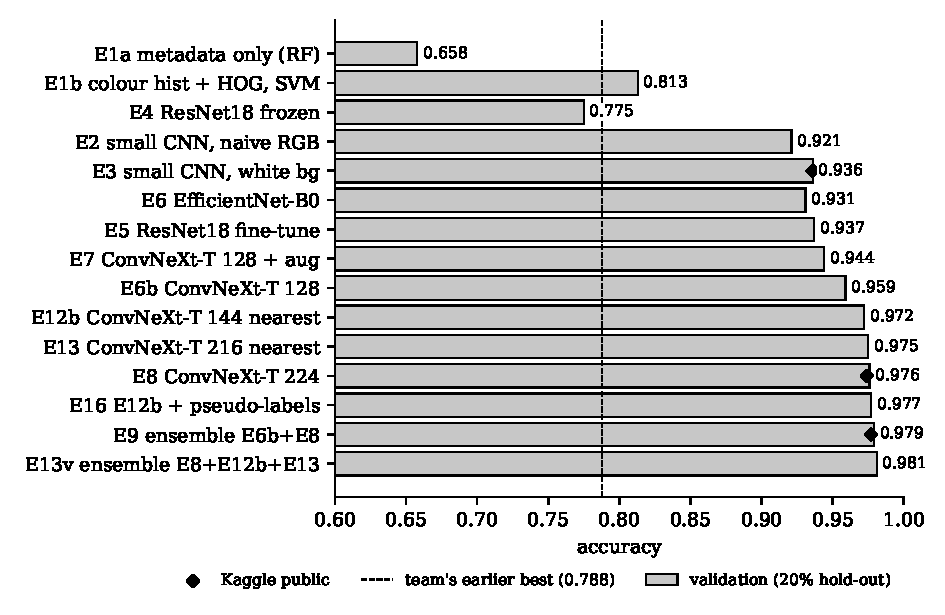
\includegraphics[width=0.9\linewidth]{accuracy_progression.pdf}
\caption{Validation accuracy of the main experiments (bars) and public Kaggle score where
submitted (diamonds). Dashed line: the team's best score before these experiments.}
\end{figure}

\section{What we learned}
\begin{enumerate}[leftmargin=*]
\item \textbf{Preprocessing matters even for a small CNN.} With identical architecture and
hyper-parameters, compositing on white instead of the default conversion gave $+1.5$ points
(E2$\to$E3), and $+2.2$ points macro precision, i.e.\ the small classes benefit most.
\item \textbf{Classical features are a solid baseline but saturate.} Colour histogram + HOG with an
SVM (0.813) already beat the team's first CNN on Kaggle, but it reaches 1.000 training accuracy:
the hand-crafted representation, not the classifier, is the bottleneck.
\item \textbf{Frozen ImageNet features fail here (0.775), worse than a CNN from scratch.}
ImageNet features describe \emph{what} the object is; this task is about \emph{how the same object
is drawn} (outline thickness, gradients, shading). Fine-tuning the whole network fixes it
($+16$ points, E4$\to$E5).
\item \textbf{Architecture: ConvNeXt-Tiny} was clearly best ($+2.2$ points over ResNet18 at the same
resolution), with the largest gains on the minority class mozilla (recall 0.85$\to$0.95).
EfficientNet-B0 gave no advantage at 128\,px and was twice as slow on the Mac.
\item \textbf{Resolution is the biggest single lever.} 128$\to$224\,px gave $+1.7$ points (E6b$\to$E8),
mostly on the classes stored natively at 240\,px (facebook 0.91$\to$0.97).
\item \textbf{Augmentation hurt} ($-1.5$ points, E7). Rotation and scaling resample the image and blur
the anti-aliased outlines that carry the vendor signature; colour jitter was deliberately not used
since colour is itself a vendor cue. Caveat: E7 changed three things at once (augmentation, label
smoothing, 15 epochs), so the loss cannot be attributed to one of them.
\item \textbf{The resize filter matters at low resolution.} At 144\,px, nearest-neighbour instead of
bicubic gave $+0.9$ points (E12a$\to$E12b), surprisingly mostly on the \emph{large} files: bicubic
downscaling also blurs crisp pixel edges. At 216--224\,px the effect disappears (E13 $\approx$ E8).
\item \textbf{More data helps}: retraining the validated recipes on 100\% of the data gave $+0.43$ (single
model, E8$\to$E10b) and $+0.24$ points (ensemble, E9$\to$E11) on Kaggle.
\item \textbf{Ensembles help only with comparably strong, diverse members.} Averaging the 128\,px and
224\,px ConvNeXt helped; adding ResNet18 or the small CNN \emph{lowered} accuracy. The final 3-model
ensemble mixes resolutions and resize filters.
\item \textbf{Pseudo-labelling} (semi-supervised): adding test images predicted with $\ge 0.99$
confidence (99.7\% correct on validation) improved a single model by $+0.5$ points (E12b$\to$E16),
but brought nothing inside the ensemble, because the pseudo-labels came from that same ensemble
(the model learns to imitate it; self-distillation).
\end{enumerate}

\section{Error analysis}
The best validation ensemble makes about 40 errors out of 1\,976 images. 32 of 41 errors of E9 are
72\,px files, often from vendors that usually ship larger files (whatsapp or facebook at 72\,px).
The most frequent confusions are whatsapp$\to$apple and facebook$\to$apple. Many of the most
confident errors are designs that are nearly identical across vendors (Figure~\ref{fig:err}), which
suggests that part of the remaining error is irreducible from the pixels alone. We also checked
other possible leaks: 349 test images are exact copies of training images, but the model already
predicts all of them correctly, and the file IDs carry no label information.

\begin{figure}[h]
\centering
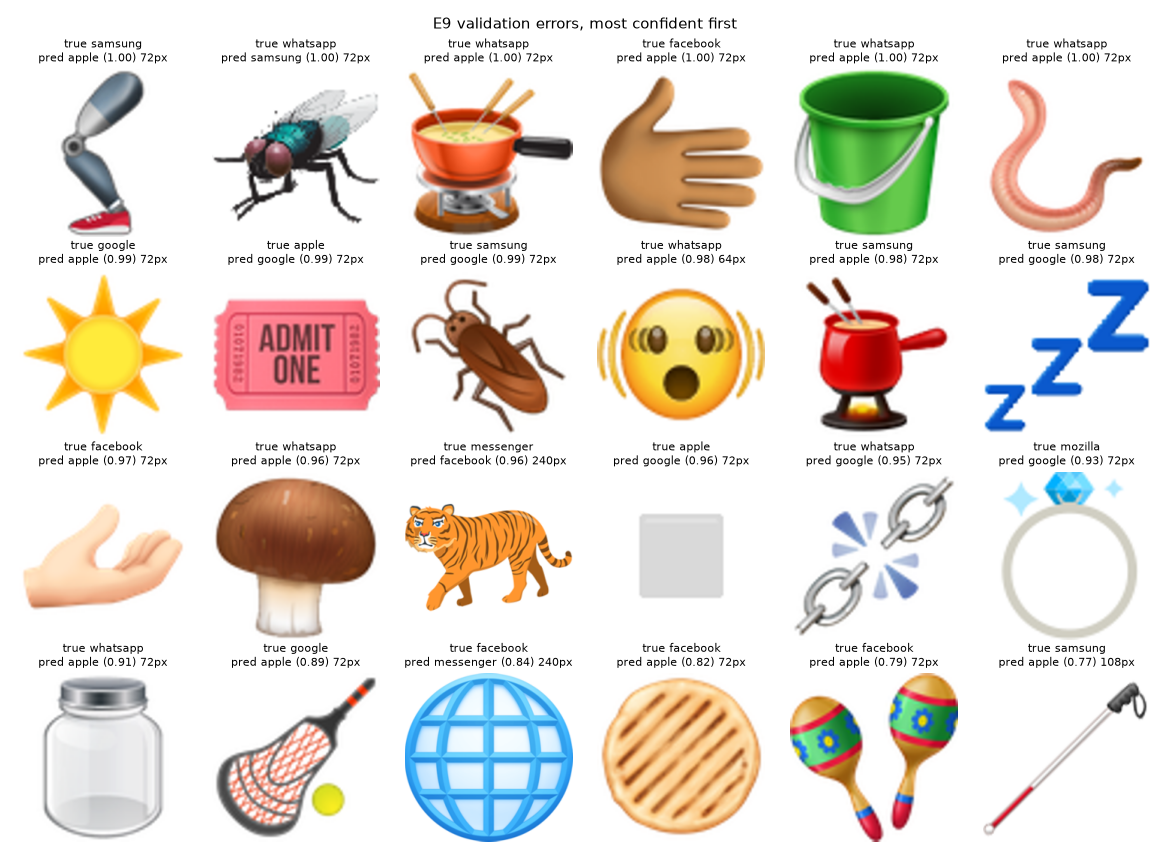
\includegraphics[width=0.78\linewidth]{e9_val_errors.png}
\caption{Most confident validation errors of E9 (true and predicted vendor, confidence, original
file size).}
\label{fig:err}
\end{figure}

\section{Final submissions}
Proposed selection for the final (private) leaderboard: \textbf{E15} (best public score, 0.981) and
\textbf{E9} (0.977) as a safety choice, since E9 is the only strong model that was validated both on
our hold-out split and on Kaggle, whereas full-data models have no held-out score.

\section{Reproducibility}
All code is in the project repository (Python, PyTorch, \code{timm}, scikit-learn; versions pinned in
\code{requirements.txt}). \code{./run\_experiments.sh E8} re-runs any experiment with its exact
command line; each run writes a JSON record, predicted probabilities and a submission file, and
\code{python -m src.results} regenerates the Excel sheet. Seed 42 is fixed for the split and the
training. GPU training on Apple MPS is not bit-exact, so re-runs can differ by about 0.2 points.
15 unit tests check the preprocessing, the split and the submission format.

\section{Limitations and possible next steps}
\begin{itemize}[leftmargin=*]
\item Larger backbones (ConvNeXt-Small/Base) and multi-seed ensembles were not tried: a 224\,px run
already takes 1.5--2 hours on the laptop. A Kaggle GPU notebook would make this feasible.
\item Only one validation split was used; 5-fold cross-validation would give more reliable
comparisons of the small differences ($<0.3$ points) between the last experiments.
\item The leader (0.998) is far above our plateau ($\approx 0.98$); given the error analysis, a much
larger model or information beyond the visual style would be needed.
\end{itemize}

\end{document}
